\documentclass[UTF8,fontset=none,12pt]{ctexart}

\setCJKmainfont{Songti SC}
\setCJKsansfont{PingFang SC}
\setCJKmonofont{Songti SC}

\usepackage[a4paper,margin=2.35cm]{geometry}
\usepackage{amsmath,amssymb,amsthm,mathtools,bm}
\usepackage{graphicx}
\usepackage{float}
\usepackage{booktabs}
\usepackage{array}
\usepackage{enumitem}
\usepackage[hidelinks]{hyperref}

\title{数值线性代数\quad 第 34 讲：Arnoldi 方法如何定位特征值}
\author{Lloyd N. Trefethen、David Bau III\quad 中文阅读版}
\date{}

\begin{document}
\maketitle
\pagestyle{plain}

Arnoldi 迭代有两重身份：它是数值线性代数中许多迭代算法的基础，更具体地说，
它还是寻找非 Hermitian 矩阵特征值的一种技术。本讲关注后一种具体作用，并在
此过程中介绍它与多项式逼近理论之间的联系；这种联系具有广泛的重要性。

\section*{用 Arnoldi 迭代计算特征值}

用 Arnoldi 迭代计算特征值的过程如下。按照上一讲算法 33.1 的描述执行迭代。
在每一步 $n$，或者每隔若干步，使用 QR 算法等标准方法计算 Hessenberg 矩阵
$H_n$ 的特征值（实际计算中，这意味着调用 EISPACK、LAPACK 或 MATLAB 提供的
软件）。这些特征值就是 Arnoldi 估计或 Ritz 值（式（33.10））。通常可以观察到
其中一些数很快收敛，而且往往是几何收敛的（即线性收敛；见习题 25.2）。一旦
它们收敛，就可以有相当把握地认为收敛值是 $A$ 的特征值。

由于可行计算中 $n\ll m$，当然不能期望通过这个过程算出 $A$ 的全部特征值。
那么 Arnoldi 迭代会找到哪些特征值？通常是极端特征值，即靠近 $A$ 的谱边缘
的特征值。幸运的是，在大多数应用中，恰恰是这些特征值最受关注。

例如，在流体力学稳定性问题中，目标是确定光滑流体流动受到小扰动后是否会
不稳定地增长；如果会，流动就可能转变为另一种更复杂的形态，甚至变成湍流。
通常的做法是将问题线性化，得到控制小扰动演化的 Jacobian 算子，然后计算该
算子在复平面中最右侧的特征值，也就是实部最大的特征值。如果这个特征值位于
右半平面，流动是不稳定的；如果它位于左半平面，流动则是稳定的。

人们已经设计了 Arnoldi 方法的许多变体，例如针对复平面上某些区域比其他区域
更重要的问题而设计的加速装置。本讲只讨论未经修饰的 Arnoldi 方法，试图说明
它为什么收敛、为什么倾向于找到 $A$ 的极端特征值，以及找到这些特征值的速度。

\section*{一个警告：非正规性}

不过首先要提醒读者一个需要谨慎对待的事实：非 Hermitian 矩阵的特征值有时
并不像人们想象的那样具有重要的物理意义。如果一个矩阵远非正规，即它的特征
向量远不正交，这意味着它的特征值条件很差，那么这些特征值可能与矩阵所控制
的物理系统实际如何变化几乎没有关系（见习题 24.3 和 26.2）。

例如，在圆管中的流体流动问题里，线性化方程的 Jacobian 可能所有特征值都在
左半平面，似乎说明流动应当稳定。然而，实际中高速管流几乎总是湍流。这个
悖论的根源在于：虽然线性化问题的所有特征模态都在衰减，但某些非模态流动
扰动仍可能被放大许多个数量级。正规矩阵或算子不会出现这种现象；对称矩阵、
Hermitian 矩阵和自伴算子都是例子。

如果一个答案对扰动高度敏感，那么你很可能问错了问题。对于涉及高度敏感特征
值的非 Hermitian 特征值计算，我们建议始终牢记这一原则。如果你是数值分析
工作者，而问题来自科学或工程领域的同事，不要不加审查地接受“真正具有物理
意义的就是这些特征值”这一保证，即使这些特征值相对于矩阵条目扰动的条件数
为 $10^4$。当然，也许确实存在高度敏感的非正规算子具有真正物理意义的情形；
但相比之下，更多情形是人们在应该进行更深层分析时，误把特征值当成了研究
对象。

\section*{Arnoldi 与多项式逼近}

设 $x$ 是 Krylov 子空间 $\mathcal K_n$（式（33.5））中的向量。它可以写成
$A$ 的各次幂作用于 $b$ 后所得向量的线性组合：

\begin{equation}
x=c_0b+c_1Ab+c_2A^2b+\cdots+c_{n-1}A^{n-1}b.
\tag{34.1}
\end{equation}

这个表达式可以简洁地描述为：它是一个关于 $A$ 的多项式乘以 $b$。也就是说，
若

\begin{equation}
q(z)=c_0+c_1z+\cdots+c_{n-1}z^{n-1},
\qquad x=q(A)b,
\tag{34.2}
\end{equation}

就得到了所需表达式；习题 33.1 已经指出了这一点。由于式（34.1）形式的每个
向量都可以写成式（34.2）的形式，Krylov 子空间迭代总可以用矩阵多项式来分析。

分析 Arnoldi 迭代的一种方式如下。定义

\[
\mathcal P^n=\{\text{次数为 $n$ 的首一多项式}\}.
\]

（“首一”是指次数为 $n$ 的项的系数为 1。）现在考虑下面的逼近问题。

\begin{center}
\fbox{\begin{minipage}{0.86\textwidth}
\textbf{Arnoldi/Lanczos 逼近问题\quad}
寻找 $p^n\in\mathcal P^n$，使得
\[
\lVert p^n(A)b\rVert=\min.
\tag{34.3}
\]
\end{minipage}}
\end{center}

和本书这一部分的其他地方一样，$\lVert\cdot\rVert=\lVert\cdot\rVert_2$。这里
在 $\mathcal P^n$ 上使用上标，是因为下一讲将讨论常数项系数 $c_0=1$、而非
最高次项系数 $c_n=1$ 的次数为 $n$ 的多项式空间；那里将使用下标。

Arnoldi 迭代有一个惊人的性质：它能够精确地解决式（34.3）。

\textbf{定理 34.1.}
只要 Arnoldi 迭代没有发生 breakdown（即 $K_n$ 具有满列秩 $n$），式（34.3）
就有唯一解 $p^n$；这个解正是 $H_n$ 的特征多项式。

\textbf{证明.}
首先注意，如果 $p\in\mathcal P^n$，那么对某个 $y\in\mathbb C^n$，有

\[
p(A)b=A^nb-Q_ny,
\]

其中 $Q_n$ 由式（33.1）定义。换句话说，式（34.3）等价于一个线性最小二乘
问题：寻找 $\mathcal K_n$ 中最接近 $A^nb$ 的点；用矩阵表示，就是寻找 $y$
使

\[
\lVert A^nb-Q_ny\rVert=\min.
\]

其解由正交条件 $p^n(A)b\perp\mathcal K_n$ 刻画，如图 34.1 所示；等价地，

\[
Q_n^*p^n(A)b=0.
\]

\begin{figure}[H]
\centering
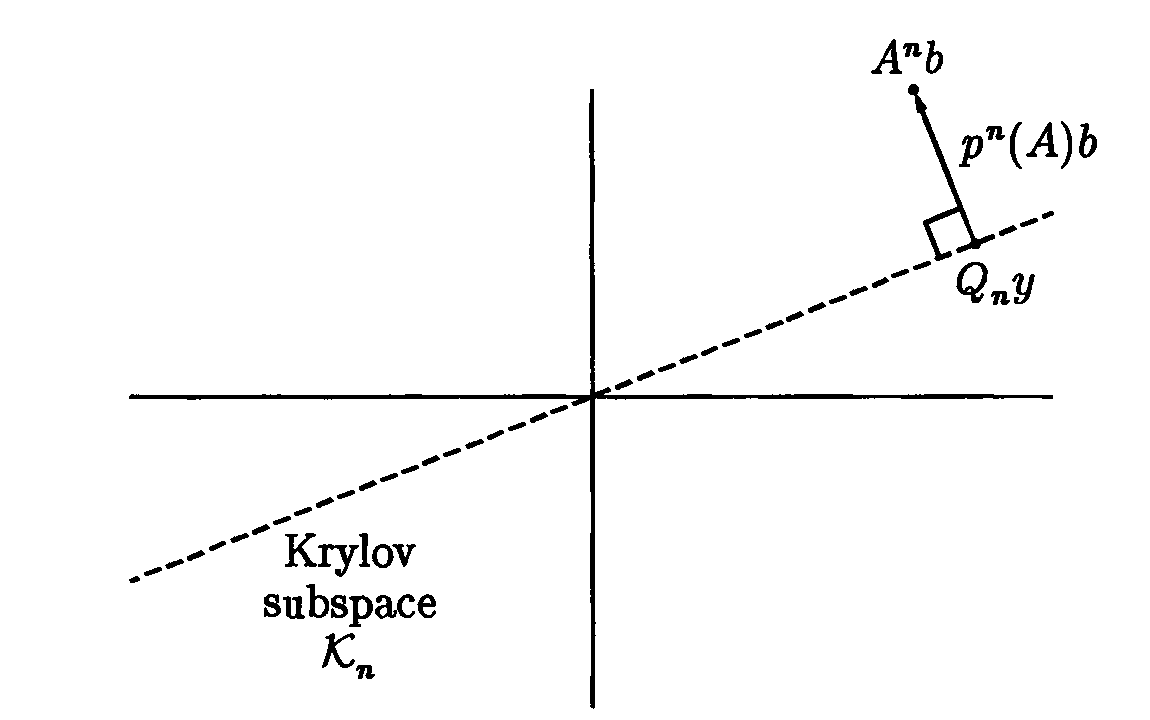
\includegraphics[width=0.78\textwidth]{../assets/figure-34-least-squares.png}
\parbox{0.78\textwidth}{\small 图 34.1. Arnoldi 迭代背后的最小二乘多项式逼近问题：$A^nb$ 到 Krylov 子空间 $\mathcal K_n$ 的正交投影为 $Q_ny$，残差为 $p^n(A)b$。}
\end{figure}

现在考虑上一讲开头提到的分解 $A=QHQ^*$。在 Arnoldi 过程的第 $n$ 步，我们
已经计算出 $Q$ 和 $H$ 的前 $n$ 列；因此存在如下形式的分解：

\[
Q=\begin{bmatrix}Q_n&U\end{bmatrix},
\qquad
H=
\begin{bmatrix}
H_n&X_1\\
X_2&X_3
\end{bmatrix},
\]

其中 $U$ 是一个 $m\times(m-n)$ 矩阵，其列正交归一且与 $Q_n$ 的列正交；
$X_1$、$X_2$、$X_3$ 的尺寸分别为 $n\times(m-n)$、$(m-n)\times n$ 和
$(m-n)\times(m-n)$，并且 $X_2$ 除右上角元素外其余元素全为 0。

正交条件变成

\[
Q_n^*Qp^n(H)Q^*b=0,
\]

这意味着 $p^n(H)$ 第一列的前 $n$ 个元素为 0。由于 $H$ 的结构，这些元素
也是 $p^n(H_n)$ 第一列的前 $n$ 个元素。根据 Cayley--Hamilton 定理，当
$p^n$ 是 $H_n$ 的特征多项式时，这些元素为 0。

反过来，假设还有另一个多项式 $p^n$ 满足 $p^n(A)b\perp\mathcal K_n$。两者
之差会给出一个次数为 $n-1$ 的非零多项式 $q$，满足 $q(A)b=0$，这与 $K_n$
满列秩的假设矛盾。\hfill$\square$

定理 34.1 给出了 Arnoldi 迭代生成的 Ritz 值的一种新解释：它们是最优多项式
（34.3）的根。

\section*{不变性}

定理 34.1 提供了一种记忆 Arnoldi 迭代基本性质的简便方式。例如，首一多项式
族 $\mathcal P^n$ 对平移 $z\mapsto z+\alpha$ 保持不变，因此 Arnoldi 迭代也
具有平移不变性。与稍后将讨论的 GMRES 等求解 $Ax=b$ 的迭代算法不同，它并
“不知道原点在哪里”。

下面总结这一点以及其他不变性。定理的每一部分都是定理 34.1 的推论，此处
不再给出证明。

\textbf{定理 34.2.}
将 Arnoldi 迭代应用于矩阵 $A\in\mathbb C^{m\times m}$，如前文所述。

\begin{description}[leftmargin=3.3cm,style=sameline]
\item[平移不变性]
若 $A$ 变为 $A+\sigma I$，其中 $\sigma\in\mathbb C$，而 $b$ 保持不变，则每一步的 Ritz 值 $\{\theta_j\}$ 变为 $\{\theta_j+\sigma\}$。

\item[尺度不变性]
若 $A$ 变为 $\sigma A$，其中 $\sigma\in\mathbb C$，而 $b$ 保持不变，则 Ritz 值 $\{\theta_j\}$ 变为 $\{\sigma\theta_j\}$。

\item[酉相似变换下的不变性]
若 $A$ 变为 $UAU^*$，其中 $U$ 为酉矩阵，同时 $b$ 变为 $Ub$，则 Ritz 值 $\{\theta_j\}$ 不变。
\end{description}

在上述三种情形中，Ritz 向量，即与 $H_n$ 的特征向量 $y_j$ 对应的向量
$Q_ny_j$，在相应变换下也保持相应的不变关系。

根据定理 24.9，每个矩阵 $A$ 都酉相似于一个上三角矩阵。因此，酉相似变换
下的不变性意味着：原则上，为了理解 Arnoldi 迭代的收敛性质，只需考虑上三角
矩阵。不过，只考虑对角矩阵还不够。在非 Hermitian（非正规）情形中，一个
矩阵包含的信息并不只有它的特征值。

\section*{Arnoldi 如何定位特征值}

现在开始回答本讲标题提出的问题。定理 34.1 说明，Arnoldi 迭代归根结底要
解决的是一个多项式逼近问题，或者等价地，一个涉及 Krylov 子空间的最小二乘
问题。如果 Arnoldi 迭代倾向于找到特征值，那么这一定是实现上述目标的副产品。

多项式逼近与 $A$ 的特征值有什么关系？稍加思考便可发现，二者之间存在如下
联系：如果目标是找到一个使 $p^n(A)$ 很小的多项式 $p^n$，一种有效办法是
让 $p^n$ 的零点靠近 $A$ 的特征值。

考虑一个极端情形。假设 $A$ 可对角化，并且只有 $n\ll m$ 个不同的特征值，
因此最小多项式次数为 $n$。由定理 34.1 可知，至少当向量 $b$ 在与每个特征
值对应的方向上都含有分量时，经过 $n$ 步便会精确找到所有这些特征值。因此，
Arnoldi 迭代在 $n$ 步后精确计算出了 $A$ 的最小多项式。

实际应用中也会发生大致相同的现象。不过此时 Ritz 值与特征值的吻合是近似而
非精确的；结果不再是最小多项式，而是一个“伪最小多项式”，即满足
$\lVert p^n(A)\rVert$ 很小的多项式 $p^n$。

\section*{Arnoldi 纽结线}

可以通过在复平面上绘制纽结线（lemniscate）来图示这一收敛过程。纽结线是一条
曲线或一组曲线：

\begin{equation}
\{z\in\mathbb C:\lvert p(z)\rvert=C\},
\tag{34.4}
\end{equation}

其中 $p$ 是多项式，$C$ 是实常数。如果 $p$ 是矩阵 $A$ 的 Arnoldi 迭代在第
$n$ 步得到的多项式 $p^n$，并取

\begin{equation}
C=\frac{\lVert p^n(A)b\rVert}{\lVert b\rVert},
\tag{34.5}
\end{equation}

那么式（34.4）定义的曲线可以称为 Arnoldi 纽结线。随着迭代次数 $n$ 增加，
通常会出现包围 $A$ 的极端特征值的纽结线分支，然后这些分支快速收缩到一点，
也就是相应的特征值本身。

为说明这些思想，令 $A$ 为一个 $m=100$ 的方阵，其元素是来自均值为 0、
标准差为 $m^{-1/2}$ 的实正态分布的独立随机数（习题 12.3）。由于 $A$ 是
实矩阵，它的特征值由实数和成对的共轭复数构成。标准差的选择使得这些特征值
大致均匀分布在单位圆盘 $\lvert z\rvert\le1$ 内。现在把角元素 $a_{11}$
改为 1.5，从而制造一个离群特征值；见图 34.2。

\begin{figure}[H]
\centering
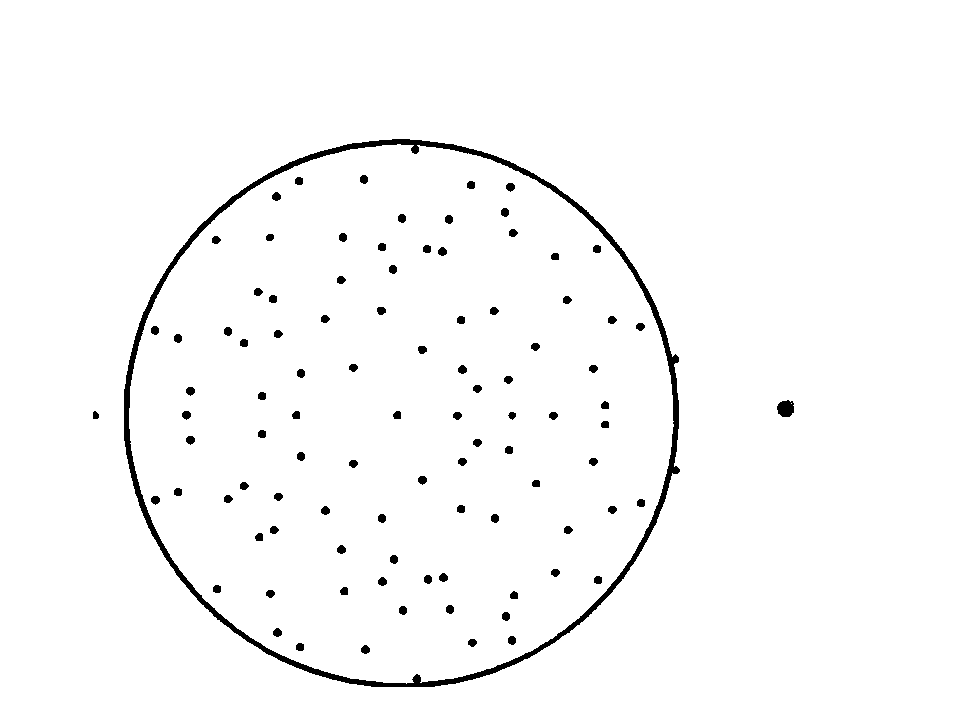
\includegraphics[width=0.63\textwidth]{../assets/figure-34-eigenvalues.png}
\parbox{0.78\textwidth}{\small 图 34.2. 一个除 $(1,1)$ 位置外均为随机元素的 $100\times100$ 矩阵 $A$ 的特征值。圆为复平面中的单位圆；特征值大致均匀分布在单位圆盘内，离群值约为 $\lambda\approx1.4852$。}
\end{figure}

从随机向量 $q_1$ 开始，对这个矩阵执行 Arnoldi 迭代。在第 $n$ 步，矩阵
$H_n$ 已经构造出来，其特征多项式反映了迭代当前掌握的谱信息。图 34.3
绘出了 $n=5,6,7,8$ 时的 Arnoldi 纽结线。在 $n=1$ 时（图中未画出），
纽结线是一个几乎不受离群特征值影响的精确圆。到 $n=5$ 时，圆开始向
$\lambda$ 的方向鼓起；到 $n=6$ 时，鼓起处收缩成颈部，并出现纽结线的新分支。
此后，这个分支在每次迭代中继续收缩。

\begin{figure}[H]
\centering
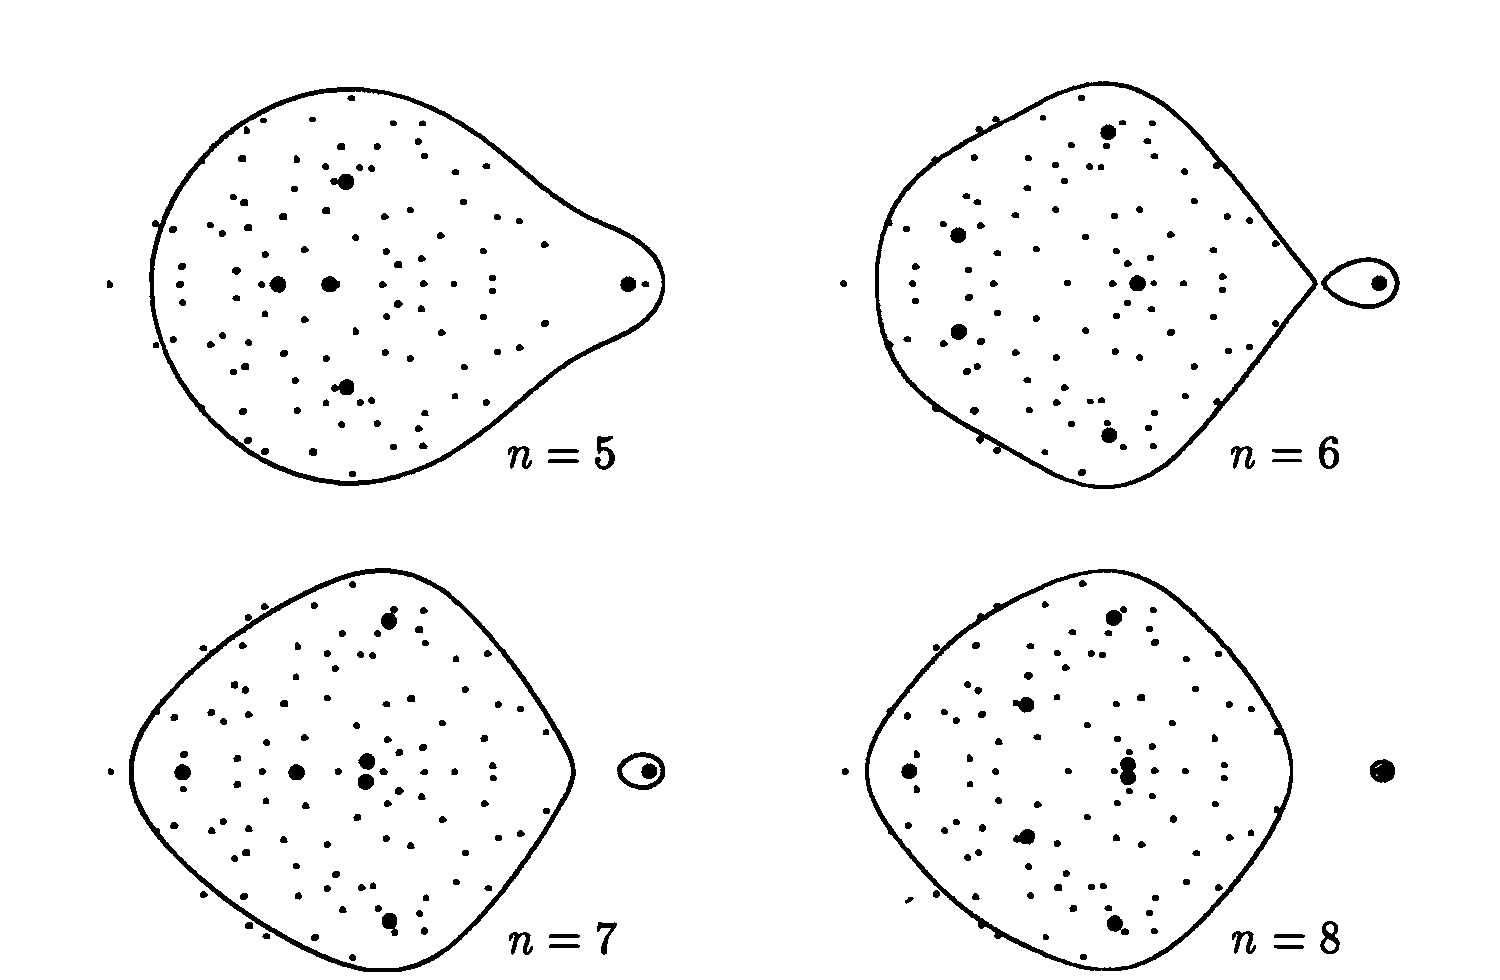
\includegraphics[width=0.90\textwidth]{../assets/figure-34-lemniscates.png}
\parbox{0.90\textwidth}{\small 图 34.3. 同一个矩阵 $A$ 在 $n=5,6,7,8$ 步的 Arnoldi 纽结线（式（34.4）–（34.5））。小点是 $A$ 的特征值，大点是 $H_n$ 的特征值，即 Ritz 值。一个纽结线分支先“吞入”离群特征值，随后以几何速率收缩到该点。}
\end{figure}

\section*{几何收敛}

在某些条件下，一些 Arnoldi 特征值估计会几何地收敛到 $A$ 的特征值。这些
问题目前尚未被完全理解，本书不在这里引用理论结果，而只考察上面的数值例子，
并给出一个部分解释。

从类似图 34.3 的图形中，无法判断超过一两位数字后的收敛速率。图 34.4
弥补了这一点：对同一个例子，绘制 $\lvert\lambda^{(n)}-\lambda\rvert$
随 $n$ 的变化，其中 $\lambda^{(n)}$ 是第 $n$ 步中最接近 $\lambda$ 的
Arnoldi 特征值估计。首先注意到，收敛显然是几何的。经过 50 次迭代，我们
已经达到 12 位精度；如果 $A$ 的维数是 1000 而不是 100，这幅图也不会有
太大差别。

\begin{figure}[H]
\centering
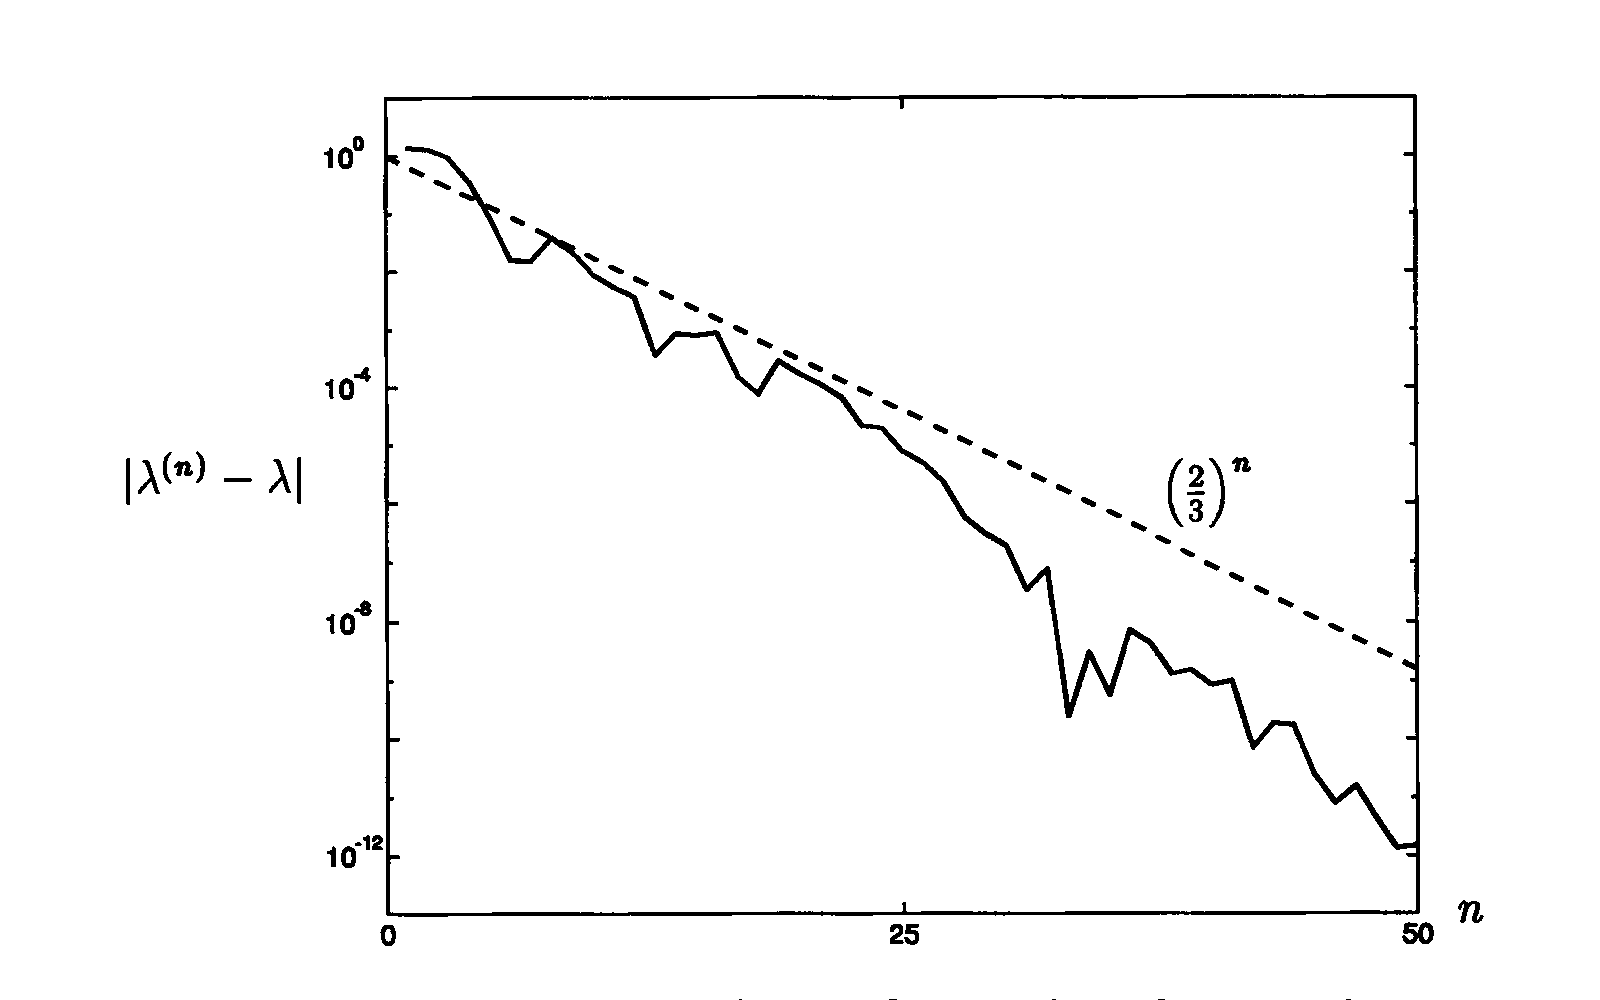
\includegraphics[width=0.88\textwidth]{../assets/figure-34-convergence.png}
\parbox{0.88\textwidth}{\small 图 34.4. 最右侧 Arnoldi 特征值估计的收敛。实线为误差 $\lvert\lambda^{(n)}-\lambda\rvert$，虚线为参考速率 $(2/3)^n$。}
\end{figure}

我们可以进行更定量的描述。至少在最初几十次迭代中，图 34.4 的收敛大致满足

\begin{equation}
\lvert\lambda^{(n)}-\lambda\rvert\approx
\left(\frac23\right)^n.
\tag{34.6}
\end{equation}

对此行为的一种解释如下。为了最小化式（34.3），$p^n$ 必须在 $A$ 的每一个
特征值处都取得大致最小的值。考虑候选多项式

\[
p(z)=z^{n-1}(z-\widetilde\lambda),
\]

其中 $\widetilde\lambda$ 是某个接近 $\lambda$ 的数。在单位圆盘内的每个
$A$ 的特征值处，$\lvert p(z)\rvert$ 都是 1 阶或更小；但在 $z=\lambda$
处，它的大小为

\[
\lvert p(\lambda)\rvert\approx
\left(\frac32\right)^n\lvert\widetilde\lambda-\lambda\rvert.
\]

（如果 $\lambda$ 恰好等于 $3/2$，这里就是等式。）当 $n$ 很大时，
$(3/2)^n$ 很大。为了使这个数仍为 1 阶，$\lvert\widetilde\lambda-\lambda\rvert$
必须足够小以抵消它，即为 $(2/3)^n$ 阶，这正是式（34.6）的结果。

图 34.4 还显示了另一个现象：经过最初几十步后，收敛开始加速，这是 Krylov
子空间迭代中常见的现象。这里发生的是，迭代开始分辨 $A$ 的其他外部特征值，
即单位圆附近的特征值。如果 $A$ 的维数为 $m=300$，那么特征值云会足够密集
地填满单位圆盘，以至于图 34.4 所示的 50 步迭代中不会出现这种加速。

\section*{习题}

\paragraph{34.1.}
给定 $A\in\mathbb C^{m\times m}$、$b\in\mathbb C^m$ 和 $p\in\mathcal P^n$，
设我们要计算 $p(A)b$。一个自然的起点是 Horner 法，可写为

\begin{equation}
p(z)=c_0+z\bigl(c_1+z\bigl(c_2+\cdots+z(c_{n-1}+z)\cdots\bigr)\bigr).
\tag{34.7}
\end{equation}

\begin{enumerate}[label=(\alph*)]
\item 根据式（34.7）写出一个 for 循环（在纸上写，不要上机），先计算 $p(A)$，
再把结果作用到 $b$ 上。确定该算法所需的运算量（保留最高阶）。
\item 另写一个计算 $p(A)b$ 的 for 循环；它要好得多，因为从一开始就把 $b$
引入计算过程。再次确定最高阶运算量。
\item 在数值分析入门教材中，推荐用 Horner 法计算多项式，因为它比先计算
$z^k$、再乘以系数 $c_k$ 并求和的直接方法更快。但对于计算 $p(A)$ 或
$p(A)b$，证明 Horner 法并不会比直接方法快很多。
\end{enumerate}

\paragraph{34.2.}
我们已经看到，Arnoldi 多项式 $p^n$ 最小化 $\lVert p^n(A)b\rVert$。另一个
可能更清楚地反映特征值信息的多项式是理想 Arnoldi 多项式，也称为 $A$ 的
Chebyshev 多项式。它定义为使 $\lVert p^*(A)\rVert$ 最小的唯一
$p^*\in\mathcal P^n$。（实践中不使用这个多项式，因为没有快速方法计算它。）

\begin{enumerate}[label=(\alph*)]
\item 证明 $p^*$ 存在。
\item 证明只要 $p^*(A)\ne0$，$p^*$ 就是唯一的。（提示：设 $p_1$ 和
$p_2$ 是给定 $A$ 和 $n$ 的两个不同的理想 Arnoldi 多项式，令
$p=(p_1+p_2)/2$，再考虑 $p(A)$ 对应于最大奇异值的奇异向量。这是一道难题。）
\end{enumerate}

\paragraph{34.3.}
令 $A$ 为 $N\times N$ 双对角矩阵，满足

\[
a_{k,k+1}=a_{k,k}=k^{-1/2},\qquad N=64.
\]

（当 $N\to\infty$ 时，$A$ 变成一个非自伴紧算子。）

\begin{enumerate}[label=(\alph*)]
\item 作图显示谱 $\Lambda(A)$ 以及 $\varepsilon$-伪谱
$\Lambda_\varepsilon(A)$ 的边界（见习题 26.1 和 26.2），其中
$\varepsilon=10^{-1},10^{-2},10^{-3},10^{-4}$。
\item 从一个随机初始向量开始，运行 Arnoldi 迭代，并在
$n=1,2,\ldots,30$ 步计算 Ritz 值。作图表示它们向 $A$ 的特征值收敛的速率，
并评论结果。
\item Arnoldi 迭代还可以用 $H_n$ 或 $\widetilde H_n$ 的伪谱来近似 $A$ 的
伪谱。在后一种情形中，$\Lambda_\varepsilon(\widetilde H_n)$ 的边界由
\[
\sigma_{\min}(zI-\widetilde H_n)=\varepsilon
\]
定义，等价地，
\[
\lVert(zI-\widetilde H_n)^{-1}\rVert=\varepsilon^{-1},
\]
其中 $I$ 是矩形版本的单位矩阵。尝试对 $n=5,10,15,20$ 绘制
$\widetilde H_n$ 的 $\varepsilon$-伪谱。它们与 $A$ 的对应伪谱有多接近？
\end{enumerate}

\end{document}
